%  LaTeX support: latex@mdpi.com 
%  For support, please attach all files needed for compiling as well as the log file, and specify your operating system, LaTeX version, and LaTeX editor.

%=================================================================
\documentclass[mathematics,article,submit,pdftex,moreauthors]{Definitions/mdpi} 
% For posting an early version of this manuscript as a preprint, you may use "preprints" as the journal and change "submit" to "accept". The document class line would be, e.g., \documentclass[preprints,article,accept,moreauthors,pdftex]{mdpi}. This is especially recommended for submission to arXiv, where line numbers should be removed before posting. For preprints.org, the editorial staff will make this change immediately prior to posting.

%--------------------
% Class Options:
%--------------------
%----------
% journal
%----------
% Choose between the following MDPI journals:
% acoustics, actuators, addictions, admsci, adolescents, aerospace, agriculture, agriengineering, agronomy, ai, algorithms, allergies, alloys, analytica, animals, antibiotics, antibodies, antioxidants, applbiosci, appliedchem, appliedmath, applmech, applmicrobiol, applnano, applsci, aquacj, architecture, arts, asc, asi, astronomy, atmosphere, atoms, audiolres, automation, axioms, bacteria, batteries, bdcc, behavsci, beverages, biochem, bioengineering, biologics, biology, biomass, biomechanics, biomed, biomedicines, biomedinformatics, biomimetics, biomolecules, biophysica, biosensors, biotech, birds, bloods, blsf, brainsci, breath, buildings, businesses, cancers, carbon, cardiogenetics, catalysts, cells, ceramics, challenges, chemengineering, chemistry, chemosensors, chemproc, children, chips, cimb, civileng, cleantechnol, climate, clinpract, clockssleep, cmd, coasts, coatings, colloids, colorants, commodities, compounds, computation, computers, condensedmatter, conservation, constrmater, cosmetics, covid, crops, cryptography, crystals, csmf, ctn, curroncol, currophthalmol, cyber, dairy, data, dentistry, dermato, dermatopathology, designs, diabetology, diagnostics, dietetics, digital, disabilities, diseases, diversity, dna, drones, dynamics, earth, ebj, ecologies, econometrics, economies, education, ejihpe, electricity, electrochem, electronicmat, electronics, encyclopedia, endocrines, energies, eng, engproc, ent, entomology, entropy, environments, environsciproc, epidemiologia, epigenomes, est, fermentation, fibers, fintech, fire, fishes, fluids, foods, forecasting, forensicsci, forests, foundations, fractalfract, fuels, futureinternet, futureparasites, futurepharmacol, futurephys, futuretransp, galaxies, games, gases, gastroent, gastrointestdisord, gels, genealogy, genes, geographies, geohazards, geomatics, geosciences, geotechnics, geriatrics, hazardousmatters, healthcare, hearts, hemato, heritage, highthroughput, histories, horticulturae, humanities, humans, hydrobiology, hydrogen, hydrology, hygiene, idr, ijerph, ijfs, ijgi, ijms, ijns, ijtm, ijtpp, immuno, informatics, information, infrastructures, inorganics, insects, instruments, inventions, iot, j, jal, jcdd, jcm, jcp, jcs, jdb, jeta, jfb, jfmk, jimaging, jintelligence, jlpea, jmmp, jmp, jmse, jne, jnt, jof, joitmc, jor, journalmedia, jox, jpm, jrfm, jsan, jtaer, jzbg, kidney, kidneydial, knowledge, land, languages, laws, life, liquids, literature, livers, logics, logistics, lubricants, lymphatics, machines, macromol, magnetism, magnetochemistry, make, marinedrugs, materials, materproc, mathematics, mca, measurements, medicina, medicines, medsci, membranes, merits, metabolites, metals, meteorology, methane, metrology, micro, microarrays, microbiolres, micromachines, microorganisms, microplastics, minerals, mining, modelling, molbank, molecules, mps, msf, mti, muscles, nanoenergyadv, nanomanufacturing, nanomaterials, ncrna, network, neuroglia, neurolint, neurosci, nitrogen, notspecified, nri, nursrep, nutraceuticals, nutrients, obesities, oceans, ohbm, onco, oncopathology, optics, oral, organics, organoids, osteology, oxygen, parasites, parasitologia, particles, pathogens, pathophysiology, pediatrrep, pharmaceuticals, pharmaceutics, pharmacoepidemiology, pharmacy, philosophies, photochem, photonics, phycology, physchem, physics, physiologia, plants, plasma, pollutants, polymers, polysaccharides, poultry, powders, preprints, proceedings, processes, prosthesis, proteomes, psf, psych, psychiatryint, psychoactives, publications, quantumrep, quaternary, qubs, radiation, reactions, recycling, regeneration, religions, remotesensing, reports, reprodmed, resources, rheumato, risks, robotics, ruminants, safety, sci, scipharm, seeds, sensors, separations, sexes, signals, sinusitis, skins, smartcities, sna, societies, socsci, software, soilsystems, solar, solids, sports, standards, stats, stresses, surfaces, surgeries, suschem, sustainability, symmetry, synbio, systems, taxonomy, technologies, telecom, test, textiles, thalassrep, thermo, tomography, tourismhosp, toxics, toxins, transplantology, transportation, traumacare, traumas, tropicalmed, universe, urbansci, uro, vaccines, vehicles, venereology, vetsci, vibration, viruses, vision, waste, water, wem, wevj, wind, women, world, youth, zoonoticdis 

%---------
% article
%---------
% The default type of manuscript is "article", but can be replaced by: 
% abstract, addendum, article, book, bookreview, briefreport, casereport, comment, commentary, communication, conferenceproceedings, correction, conferencereport, entry, expressionofconcern, extendedabstract, datadescriptor, editorial, essay, erratum, hypothesis, interestingimage, obituary, opinion, projectreport, reply, retraction, review, perspective, protocol, shortnote, studyprotocol, systematicreview, supfile, technicalnote, viewpoint, guidelines, registeredreport, tutorial
% supfile = supplementary materials

%----------
% submit
%----------
% The class option "submit" will be changed to "accept" by the Editorial Office when the paper is accepted. This will only make changes to the frontpage (e.g., the logo of the journal will get visible), the headings, and the copyright information. Also, line numbering will be removed. Journal info and pagination for accepted papers will also be assigned by the Editorial Office.

%------------------
% moreauthors
%------------------
% If there is only one author the class option oneauthor should be used. Otherwise use the class option moreauthors.

%---------
% pdftex
%---------
% The option pdftex is for use with pdfLaTeX. If eps figures are used, remove the option pdftex and use LaTeX and dvi2pdf.

%=================================================================
% MDPI internal commands
\firstpage{1} 
\makeatletter 
\setcounter{page}{\@firstpage} 
\makeatother
\pubvolume{1}
\issuenum{1}
\articlenumber{0}
\pubyear{2022}
\copyrightyear{2022}
%\externaleditor{Academic Editor: Firstname Lastname}
\datereceived{} 
%\daterevised{} % Only for the journal Acoustics
\dateaccepted{} 
\datepublished{} 
%\datecorrected{} % Corrected papers include a "Corrected: XXX" date in the original paper.
%\dateretracted{} % Corrected papers include a "Retracted: XXX" date in the original paper.
\hreflink{https://doi.org/} % If needed use \linebreak
%\doinum{}
%------------------------------------------------------------------
% The following line should be uncommented if the LaTeX file is uploaded to arXiv.org
%\pdfoutput=1

%=================================================================
% Add packages and commands here. The following packages are loaded in our class file: fontenc, inputenc, calc, indentfirst, fancyhdr, graphicx, epstopdf, lastpage, ifthen, lineno, float, amsmath, setspace, enumitem, mathpazo, booktabs, titlesec, etoolbox, tabto, xcolor, soul, multirow, microtype, tikz, totcount, changepage, attrib, upgreek, cleveref, amsthm, hyphenat, natbib, hyperref, footmisc, url, geometry, newfloat, caption

%%% ДЛЯ РУССКОГО ТЕКСТА закомментировать потом!
\usepackage{inputenc}
\usepackage[T2A,T1]{fontenc}
\usepackage[english,russian]{babel}
\usepackage{cmap}
%%%


%=================================================================
%% Please use the following mathematics environments: Theorem, Lemma, Corollary, Proposition, Characterization, Property, Problem, Example, ExamplesandDefinitions, Hypothesis, Remark, Definition, Notation, Assumption
%% For proofs, please use the proof environment (the amsthm package is loaded by the MDPI class).

%=================================================================
% Full title of the paper (Capitalized)
\Title{Using the ... Algorithm to Detect Kinetic Parameters of Catalytic Isomerization of the Pentane-Hexane Fraction}
% Дежурное название: Использование ...алгоритма для определения кинетических параметров процесса каталитической изомеризации пентан-гексановой фракции
% Еще один вариант: О решении задачи определения Kinetic Parameters of Catalytic Isomerization of the Pentane-Hexane Fraction с помощью Parallel Global Search Algorithm
% На английском: About Solving the Problem of Finding Kinetic Parameters of Catalytic Isomerization of the Pentane-Hexane Fraction Using Parallel Global Search Algorithm

% MDPI internal command: Title for citation in the left column
\TitleCitation{Title}

% Author Orchid ID: enter ID or remove command
\newcommand{\orcidauthorA}{0000-0001-5273-2471} % Add \orcidA{} behind the author's name
\newcommand{\orcidauthorB}{0000-0002-8736-0652} % Add \orcidB{} behind the author's name
\newcommand{\orcidauthorC}{0000-0003-4219-4870} 

% Authors, for the paper (add full first names)
\Author{Konstantin Barkalov $^{1}$\orcidA{}, Irek Gubaydullin $^{2,3}$, Ilya Lebedev $^{1}$\orcidB{}, Roza Faskhutdinova $^{2,3}$ and Leniza Enikeeva $^{3,4,}$*\orcidC{}}

%\longauthorlist{yes}

% MDPI internal command: Authors, for metadata in PDF
\AuthorNames{Konstantin Barkalov, Irek Gubaydullin, Ilya Lebedev, Roza Faskhutdinova and Leniza Enikeeva}

% MDPI internal command: Authors, for citation in the left column
\AuthorCitation{Barkalov, B.; Gubaydullin, I.; Lebedev, I.; Faskhutdinova, R.; Enikeeva, L.}
% If this is a Chicago style journal: Lastname, Firstname, Firstname Lastname, and Firstname Lastname.

\address{%
$^{1}$ \quad Lobachevsky State University of Nizhny Novgorod, Nizhny Novgorod, Russia; konstantin.barkalov@itmm.unn.ru\\
$^{2}$ \quad Institute of Petrochemistry and Catalysis – Subdivision of the Ufa Federal Research Centre of RAS, Ufa, Russia; irekmars@mail.ru \\
$^{3}$ \quad Ufa State Petroleum Technological University, Ufa, Russia; roza\_fask@mail.ru\\
$^{4}$ \quad Novosibirsk State University, Novosibirsk, Russia; leniza.enikeeva@yandex.ru
}

% Contact information of the corresponding author
\corres{Correspondence: leniza.enikeeva@yandex.ru (E.L.); konstantin.barkalov@itmm.unn.ru (B.K.) }

% Current address and/or shared authorship
%\firstnote{Current address: Affiliation 3.} 
%\secondnote{These authors contributed equally to this work.}
% The commands \thirdnote{} till \eighthnote{} are available for further notes

%\simplesumm{} % Simple summary

%\conference{} % An extended version of a conference paper

% Abstract (Do not insert blank lines, i.e. \\) 
\abstract{A single paragraph of about 200 words maximum. For research articles, abstracts should give a pertinent overview of the work. We strongly encourage authors to use the following style of structured abstracts, but without headings: (1) Background: place the question addressed in a broad context and highlight the purpose of the study; (2) Methods: describe briefly the main methods or treatments applied; (3) Results: summarize the article's main findings; (4) Conclusions: indicate the main conclusions or interpretations. The abstract should be an objective representation of the article, it must not contain results which are not presented and substantiated in the main text and should not exaggerate the main conclusions.}

% Keywords
\keyword{kinetic model; inverse problems of chemical kinetics; mathematical modeling; catalytic isomerisation of pantane-hexane fraction (List three to ten pertinent keywords specific to the article; yet reasonably common within the subject discipline.)} 


% The fields PACS, MSC, and JEL may be left empty or commented out if not applicable
%\PACS{J0101}
%\MSC{}
%\JEL{}

%%%%%%%%%%%%%%%%%%%%%%%%%%%%%%%%%%%%%%%%%%
% Only for the journal Diversity
%\LSID{\url{http://}}

%%%%%%%%%%%%%%%%%%%%%%%%%%%%%%%%%%%%%%%%%%
% Only for the journal Applied Sciences
%\featuredapplication{Authors are encouraged to provide a concise description of the specific application or a potential application of the work. This section is not mandatory.}
%%%%%%%%%%%%%%%%%%%%%%%%%%%%%%%%%%%%%%%%%%

%%%%%%%%%%%%%%%%%%%%%%%%%%%%%%%%%%%%%%%%%%
% Only for the journal Data
%\dataset{DOI number or link to the deposited data set if the data set is published separately. If the data set shall be published as a supplement to this paper, this field will be filled by the journal editors. In this case, please submit the data set as a supplement.}
%\datasetlicense{License under which the data set is made available (CC0, CC-BY, CC-BY-SA, CC-BY-NC, etc.)}

%%%%%%%%%%%%%%%%%%%%%%%%%%%%%%%%%%%%%%%%%%
% Only for the journal Toxins
%\keycontribution{The breakthroughs or highlights of the manuscript. Authors can write one or two sentences to describe the most important part of the paper.}

%%%%%%%%%%%%%%%%%%%%%%%%%%%%%%%%%%%%%%%%%%
% Only for the journal Encyclopedia
%\encyclopediadef{For entry manuscripts only: please provide a brief overview of the entry title instead of an abstract.}

%%%%%%%%%%%%%%%%%%%%%%%%%%%%%%%%%%%%%%%%%%
\begin{document}

%%%%%%%%%%%%%%%%%%%%%%%%%%%%%%%%%%%%%%%%%%
\section{Introduction}


%Часть ННГУ - начало

In the complex problems of chemical kinetics, kinetic constants of reactions cannot be found analytically, they can only be found using numerical methods (see, for example, \cite{Zaynullin2020,Enikeeva2020,Koledina2019}). In this case, the quality criterion (objective function) is set in the form of a certain algorithm, which includes the stage of numerical modeling, which, in turn, makes it compute-intensive. Furthermore, in the inverse problems of chemical kinetics, the objective function can be substantially multiextremal, i.e., having many local extremes along the global one. 

Numerical methods for solving such multiextremal problems (global optimization methods) differ significantly from local optimization methods since they require the study of the entire search domain (see, for example, \cite{PaulaviciusZilinskas2014,Sergeyev2017}). These methods can be divided into two classes: meta-heuristic and deterministic. Metaheuristic algorithms are usually based on simulations of processes occurring in the wild.
Examples of metaheuristic algorithms are simulated annealing, evolution and genetic algorithms, etc. (see, for example, \cite{Battiti2009,Eiben2015}).
These algorithms are included in many software libraries for solving global optimization problems (for example, MATLAB Global Optimization Toolbox, Scipy.Optimize, etc.).
Due to the operation speed and low requirements for computing resources (in particular, memory), metaheuristic algorithms have become widespread for solving practical problems. However, the solution to the problem found by such an algorithm is, in general, local and can be located far from the global optimum \cite{Kvasov2018}. 

It is also possible to construct deterministic methods of global search, which are different from brute force algorithms and metaheuristic algorithms. Such methods are associated with the presence and consideration of a priori assumptions about the problem properties. 
One of the natural assumptions about the problem is that changing the values of an objective function is limited by changes of its argument. In this case, the function satisfies the Lipschitz condition, and the problem itself is called the Lipschitz global optimization problem. The central direction of the development of modern methods of Lipschitz optimization is the development of parallel algorithms. It is assumed that the values of the objective function are determined as a result of solving some other task and require a costly computational experiment.


This paper reflects the results of applying parallel methods of Lipschitz optimization developed in \cite{Barkalov2016,Strongin2018,Sysoyev2017}, to the solution of inverse problems of chemical kinetics.  
The main part of the paper is structured as follows. 
Section 2 provides a description of the mathematical model of the chemical reaction under study. Section 3 discusses the standard formulation of the Lipschitz global optimization problem and the algorithm for solving it. It also outlines the issues related to the technical aspects of the implementation of the parallel algorithm. The results of the numerical solution of the inverse problem of chemical kinetics using the developed parallel algorithm are discussed in Section 4. The last section contains the conclusion and plans for future work.

%Часть ННГУ - конец

\section{Mathematical model}

Let's consider the scheme of chemical transformations of the isomerization of the pentane-hexane fraction. The reaction consists of 48 reaction stages, ... 

2-MP is 2-methyl pentane; 

3-MP is 3-methyl pentane; 

2,2-DMB is 2,2-dimethyl butane; 

2,3-DMB is 2,3-dimethyl butane

CH* is cyclohexane

MCP is methyl cyclopentane

B is benzene.

3-MP is 3-methyl pentane; 

2,2-DMB is 2,2-dimethyl butane; 

2,3-DMB is 2,3-dimethyl butane

CH* is cyclohexane


\begin{table}[H] 
\caption{Transformations of the catalytic isomerization of the pentane-hexane fraction.\label{tab11}}
\newcolumntype{C}{>{\centering\arraybackslash}X}
\begin{tabularx}{\textwidth}{CCCC}
\toprule
\textbf{No}	& \textbf{Reaction}	& \textbf{E, kJ/mol}     & \textbf{log($k_0$)} \\
\midrule
1	& $n$-C$_5$H$_{12}$ $\rightarrow$ $iso$-C$_5$H$_{12}$ & 149.320 & 18.492\\
2 & $iso$-C$_5$H$_{12}$ $\rightarrow$ $n$-C$_5$H$_{12}$ & 160.474 & 19.507 \\
3 & $n$-C$_6$H$_{14}$ $\rightarrow$ 2-MP & 102.833 & 8.127 \\
4 & 2-MP $\rightarrow$ $n$-C$_6$H$_{14}$ & 106.317 & 11.279 \\

\bottomrule
\end{tabularx}
\end{table}


The introduction should briefly place the study in a broad context and highlight why it is important. It should define the purpose of the work and its significance. The current state of the research field should be reviewed carefully and key publications cited. Please highlight controversial and diverging hypotheses when necessary. Finally, briefly mention the main aim of the work and highlight the principal conclusions. As far as possible, please keep the introduction comprehensible to scientists outside your particular field of research. Citing a journal paper \cite{ref-journal}. Now citing a book reference \cite{ref-book1,ref-book2} or other reference types \cite{ref-unpublish,ref-communication,ref-proceeding}. Please use the command \citep{ref-thesis,ref-url} for the following MDPI journals, which use author--date citation: Administrative Sciences, Arts, Econometrics, Economies, Genealogy, Humanities, IJFS, Journal of Intelligence, Journalism and Media, JRFM, Languages, Laws, Religions, Risks, Social Sciences, Literature.


%Часть ННГУ - начало
\section{Parallel Algorithm for Solving Global Optimization Problems }\label{Sec_GSA}

\subsection{Statement of the global optimization problem}

As mentioned above, from a mathematical point of view, the inverse problem of chemical kinetics can be considered a Lipschitz global optimization problem. 
In general, the problem of the specified class can be formulated as follows:
\begin{gather}
 \phi^* = \phi(y^\ast)=\min{\left\{\phi(y):y\in D\right\}}, \label{problemN}\\
 D=\left\{y\in R^N: a_i\leq y_i \leq b_i, \;  1\leq i \leq N\right\} \label{D},
\end{gather}
where $a,b \in R^N$ are boundaries of the search domain, and the objective function $\phi(y)$ satisfies the Lipschitz condition
\begin{equation}\label{Lip}
\left|\phi(y_1)-\phi(y_2)\right|\leq L\left\|y_1-y_2\right\|,\; y_1,y_2 \in D.
\end{equation}

The function $\phi(y)$ is assumed to be multiextremal and is given in the form of some computational algorithm. The input of this algorithm is supplied with a parameter vector, and the output is the corresponding value of the function. Such functions are often referred to as ``black-box'' functions. It is also assumed that each calculation of the function value at the search domain point (hereinafter also referred to as trial) is a laborious operation and requires significant computational resources. As noted in the introduction, this statement of the problem fully corresponds to the inverse problem of chemical kinetics.

The Lipschitz condition (\ref{Lip}) can be used to construct estimates of the function global minimum, which can serve as a foundation for designing global optimization algorithms and proving their convergence conditions (see, for example, \cite{Strongin2000}).

One of the main difficulties in solving Lipschitz global optimization problems is the so-called ``curse of dimensionality'' --- the exponential increase in the number of trials required to solve a problem with a given accuracy, accompanied by the increasing dimensionality of the problem. It is possible to smooth this effect while maintaining the accuracy of the solution by constructing significantly uneven coverages of the search domain with trial points.

Known examples of such methods are the non-uniform space covering method \cite{Evtushenko2013}, the simplicial partitions method \cite{PaulaviciusZilinskas2014}, the diagonal partitions method \cite{Sergeyev2017}. These techniques are based on adaptive partitioning of the search domain into a finite number of subdomains at each iteration.
Then the need for further subdivision for a more detailed study of these subdomains is estimated (using the accumulated information about the objective function). 
A fundamentally different approach to solving a multidimensional problem (\ref{problemN}) is its reduction to one or more one-dimensional problems followed by the use of efficient methods of one-dimensional optimization. Such reduction may be accomplished, for example, by a nested optimization scheme \cite{Grishagin2018} or by Peano-Hilbert curves \cite{Barkalov2018}. The latter approach is used in this work.

Using a continuous single-valued mapping (Peano-Hilbert curve) $y(x)$ of the real axis segment $[0,1]$ onto hyperinterval $D$ from (\ref{D}), a multidimensional problem (\ref{problemN}) can be reduced to a one-dimensional one
\[
\phi(y^\ast)=\phi(y(x^\ast))=\min{\left\{\phi(y(x)): x\in[0,1]\right\}}.
\]
It is known \cite{Strongin2000, Sergeyev2013} that the reduced one-dimensional function $\phi(y(x))$ will no longer be Lipschitzian, but will satisfy the H{\"o}lder condition
\[
\left|\phi(y(x_1))-\phi(y(x_2))\right|\leq H\left|x_1-x_2\right|^{1/N},
\]
where the H{\"o}lder constant $H$ is associated with the Lipschitz constant $L$ by the relationship $ H=2 L \sqrt{N+3}$.

Specific methods of numerical construction of this kind of mappings (called evolvents) are discussed in \cite{Strongin2000,Sergeyev2013}.
Here we note that evolvent will approximate the theoretical Peano-Hilbert curve with an accuracy of $2^{-m}$, where $m$ is the parameter that sets the approximation accuracy. Examples of evolvent for different dimensions are shown in Fig.~\ref{fig:Peano}.

\begin{figure}
\center
\begin{minipage}{0.45\linewidth}
\center{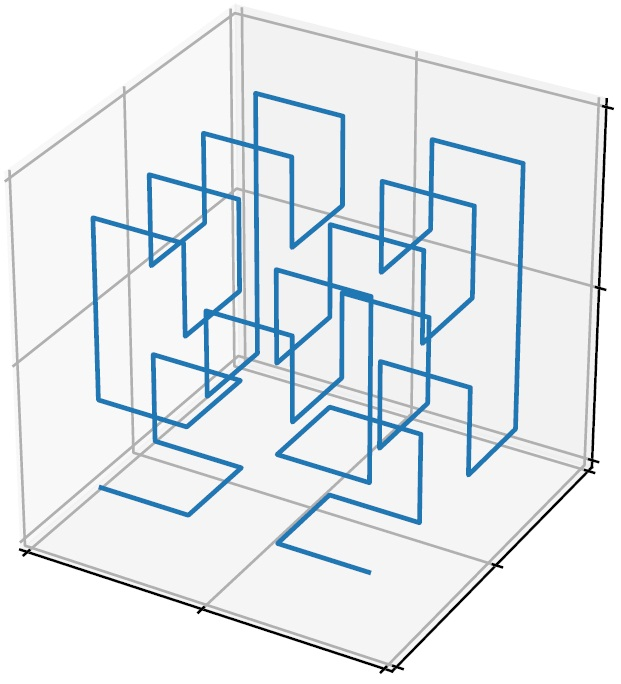
\includegraphics[width=0.9\linewidth]{fig1a.JPG} \\ (a)}
\end{minipage}
\begin{minipage}{0.45\linewidth}
\center{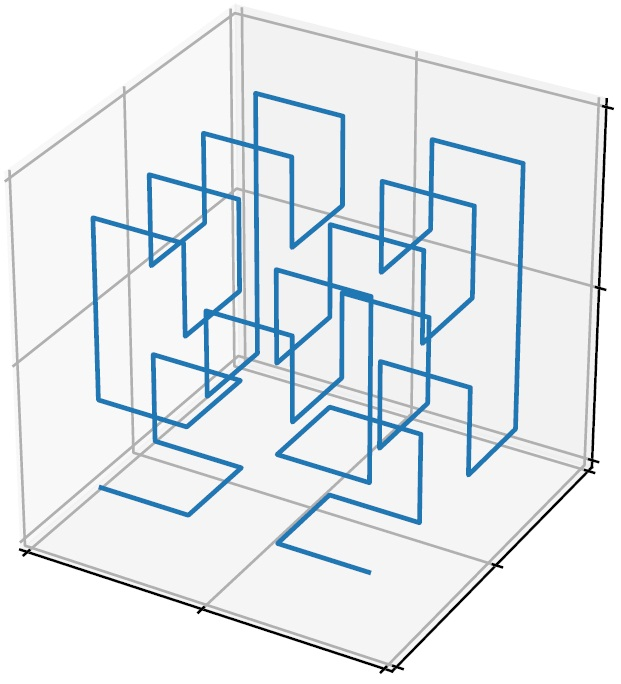
\includegraphics[width=0.9\linewidth]{fig1b.JPG} \\ (b)}
\end{minipage}
\caption{Evolvents with $m=4$ and (a) $N=2$, (b) $N=3$.}\label{fig:Peano}
\end{figure}   


Thus, under this approach, the search trial at some point $x^k\in[0,1]$ will include the construction of the image $y^k=y(x^k)$ first, and only then the calculation of the value of the function $ z^k = \phi(y^k)$.
We will call the three values $\{x^k,y ^k,z^k\}$ the trial result.

%поправить название
\subsection{Asynchronous parallel algorithm used to determine the global minimum of a function}

The parallel algorithm used in this study is based on the information and statistical approach to the development of global optimization methods, the theoretical foundations of which are set out in \cite{Strongin2000}. 

We have implemented an asynchronous paralleling scheme of the ``master/worker'' type. The master process performs a global search algorithm, in which the search information is accumulated. Then the Lipschitz constants for the objective function are estimated on its basis, and the points of new trials are calculated and distributed over the work processes. Worker-processes receive points from the master, carry out new trials in them, and send the results of the trials to the master. 

Let us assume that at each iteration, the master-process calculates one point of the new trial and transfers it for testing to the worker-process. At the same time, a trial performed by a worker is a much more labor-intensive operation than selection of a new point by a master, which eliminates the downtime of worker-processes. 
In this case (unlike synchronous parallel algorithms), the total number of trials performed by each worker-process  will depend on the labor intensity of the specific trial and cannot be estimated in advance.

When describing a parallel algorithm, let us assume that there is one process master and $p$ workers. The upper index will indicate the serial number of the trial performed, and the lower index will be used to number the trials in ascending order of the coordinate.
 
The initial iteration is carried out according to a special rule. The master process (let us assume that this is the process No 0) initiates  $p$ parallel trials at $p$ different points of the search domain, two of which are boundary points, and the rest are arbitrary internal points (for example, uniformly distributed). Thus, the initial trials are carried out at the points $\{y(x^1), y(x^2), ...,y(x^p)\}$, where $x^1 = 0$, $x^p = 1$, $x^i\in(0,1), i=2,..., p-1$.

Let us suppose that the master-process has obtained the results of $k$ trials, and at the current time the worker-processes are conducting trials at the points
$\{y(x^{k+1}), y(x^{k+2}), ...,y(x^{k+p})\}$.

Let one of the processes (without limiting the commonality, we can assume that this is the process No 1), at some point in time complete the trial at the point $y(x^{k+1})$.
The remaining processes are at the stage of conducting their trials, i.e. at these points multiple trials have already started, but have not yet been completed.

Then the No 1 process forwards to the master process the trial results, i.e. the three values $\{x^{k+1},y^{k+1},z^{k+1}\}$.
The master saves the results in its information base and selects a new trial point $x^{k+p+1}$ for the process No 1 in accordance with the rules described below.

Step 1. Renumber he point of the set 
\[
X_k = \left\{x^1, x^2,...,x^{k+p} \right\},
\]
which contains all the points at which the trials either have been carried out or are being carried out by the lower index in ascending order, i.e.
\[
0=x_1<x_2<...<x_{x+p}=1.
\]
Step 2. Calculate values
\[
M_1=\max \left\{ \frac{ \left|z_i - z_{i-1} \right|}{(x_i-x_{i-1})^{1/N}} : x_{i-1} \notin I_k, x_i \notin I_k, 2\leq i\leq k+p \right\},
\]
\[
M_2=\max \left\{ \frac{ \left|z_{i+1} - z_{i-1} \right|}{(x_{i+1}-x_{i-1})^{1/N}} : x_i \in I_k, 2\leq i < k+p \right\},
\]
\[
M=\max\{M_1,M_2\},
\]
where $z_i=\phi(y(x_i))$, if $x_i \notin I_k, \; 1\leq i \leq k+p$. The $z_i$ values at $x_i \in I_k$ are undefined because the trials at $x_i \in I_k$ are not yet complete. If the value $M$ is 0, assign $M=1$.

Step 3. For each interval $(x_{i-1},x_i), \; x_{i-1} \notin I_k, x_i \notin I_k, \; 2\leq i\leq k+p$, calculate the value 
\[
R(i)=rM\Delta_i+\frac{(z_i-z_{i-1})^2}{rM\Delta_i}-2(z_i+z_{i-1}),
\]
called the characteristic of this interval. Here $\Delta_i=\left(x_i-x_{i-1}\right)^{1/N}$, and $r>1$ is the reliability parameter of the method.

Step 4. Select the interval $[x_{t-1},x_t]$ with the highest characteristic value, i.e.
\[
R(t) = \max \left\{ R(i): \; x_{i-1} \notin I_k, x_i \notin I_k, \; 2\leq i\leq k+p \right\}.
\]

Step 5. Calculate the point $x^{k+p+1} \in (x_{t-1},x_t)$ according to the formula
\[
x^{k+p+1} = \frac{x_{t}+x_{t-1}}{2} - \mathrm{sign}(z_{t}-z_{t-1})\frac{1}{2r}\left[\frac{\left|z_{t}-z_{t-1}\right|}{M}\right]^N.
\]

Immediately after calculating the point $x^{k+p+1}$ of the next trial, the master-process adds it to the set $I_k$ and forwards it to the worker-process, which initiates the trial at this point. 

The master process terminates the algorithm if either the condition $\Delta_{t}<\varepsilon$ ($t$ is number of the interval with the maximum characteristic from Step 4) or the condition $k>K_{max}$ ($k$ is the number of trials performed) is met.
The real number $\varepsilon>0$ and the integer $K_{max}>0$ are the algorithm parameters which correspond to the accuracy of the solution search and the maximum number of trials.

The sequential global search algorithm, on the basis of which the proposed asynchronous algorithm was implemented, allows the following interpretation \cite{Molinaro2001}. Using the points of previously performed trials, it is possible to construct a minorant of the objective function, for which the value $-R(i)$, where $R(i)$ is the value of the characteristic of the interval $(x_{i-1}, x_i)$, will be the value of the minorant at the point of its minimum at the interval $(x_{i-1},x_i), 1\leq i\leq k+p$. In accordance with Step 4 of the algorithm, a new trial is carried out in the interval with the lowest value of the minorant. And in accordance with Step 5, the point of the new trial coincides with the minorant minimum point.

The theory of convergence and various modifications of serial and parallel algorithms are detailed in the monographs \cite{Strongin2000,Sergeyev2017}. 
It should be noted that the asynchronous parallelization scheme described here, in contrast to the synchronous schemes used earlier in solving a number of application problems (see \cite{Kalyulin2017, Modorskii2016}), provides a full load of all the processes involved in solving problems with different labor intensity of trials at different points in the search domain.


\subsection{Features of the software implementation of the parallel algorithm}

\begin{figure}
\center{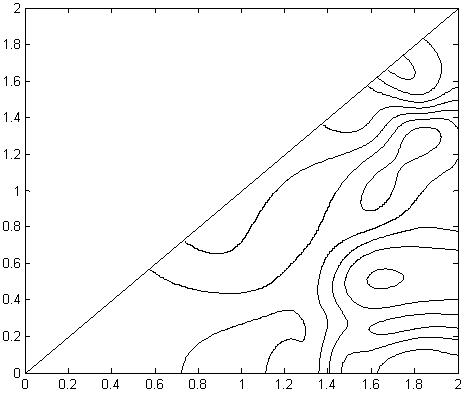
\includegraphics[width=0.9\linewidth]{fig2.JPG}}
\caption{Implemented scheme of parallel computations (1 -- link via MPI, 2 -- link via streams).}\label{fig:Impl}
\end{figure}   

In our implementation of the global search algorithm, MPI is used to organize parallel calculations. A process with the rank 0 acts as a master, processes with a rank other than 0 act as calculators (workers), see the description of the algorithm in the previous section.

The principle of process interaction (Figure \ref{fig:Impl}, link 1) is as follows. The first step in the master-process is to select $p$ points for trials. The selected trial points are sent to the calculators and the master enters the stand-by state for receiving messages. Messages from the calculators contain the trial result. The obtained information is used to select the point of the next trial. The new point is sent as a message to the calculator. If the stopping condition is met in the algorithm, instead of the trial point the master sends a shutdown message to the calculator.

Each process that performs the role of a calculator creates an instance of the task when it starts, and then goes into a stand-by mode for messages from the master-process. When a message containing a trial point is received, a computational experiment is performed. The results of the experiment are sent to the master. After the experiment, the process itself continues to wait for new messages. When a shutdown message is received, the resources used by the task are released and the main process is terminated.

When implementing the asynchronous scheme, we assumed that the start time of calculating the objective function values is different for each particular process. Our implementation takes into account the fact that the trial point as well as the calculation results represent a small amount of data that can be sent relatively quickly over the network. As a result, basic point-to-point MPI message forwarding operations were used to interact between the master and the calculators (Figure \ref{fig:Impl}, link 1). 

When conducting computational experiments (see next section), the solution of the direct problem of chemical kinetics was performed using MATLAB. In the initial version of the problem, each set of parameters required starting the MATLAB process, transferring the trial point, as well as obtaining the results of computational experiments. A number of additional settings have been made to reduce computing overhead. First, the source code for the computational experiment was compiled into an executable application. Second, the approach in which MATLAB receives a trial point through input stream, and returns the results of computational experiment through output stream was implemented. This approach allowed each calculator to run a process with compiled MATLAB code once, intercept input and output streams, and then perform calculations without waiting for new processes to start. 

\section{Numerical Experiments}

The asynchronous parallel global search algorithm was implemented on C++; the software was built on Intel MPI and Intel C++ compiler, version 2017.0.1. The objective function of the problem to be solved was implemented in MATLAB 2019b.
In order to check the stability of the developed parallel program, it was launched on three different supercomputers: Lomonosov-2 (Moscow State University), Lobachevsky (University of Nizhni Novgorod), and MVS-10P (Joint Supercomputer Center of the RAS). The main part of the experiments was carried out on the Lomonosov-2 supercomputer with the following computer nodes characteristics: Intel Haswell-EP E5-2697v3 CPU (processor frequency 2.6 GHz, 14 cores), 64 GB of RAM, CentOS 7 operating system.

To solve the optimization problem, a combination of the parallel global search algorithm and a local optimization method was used. In the first stage of the search, the parallel asynchronous algorithm described in Section \ref{Sec_GSA} was used. 101 processes were involved in the launch, of which one process was a master and the remaining 100 were workers (calculators). The values of the method parameters were set as follows: the maximum number of trials $K_{max}=3000$, the search accuracy $\varepsilon=10^{-3}$, the reliability parameter $r=3$, the evolvent accuracy parameter $m=12$. At the second stage, the solution was refined using the pattern search method with an accuracy of $\varepsilon=10^{-4}$ and a limit on the number of trials $K_{max}=500$.
The total time for solving the problem was 8109 seconds, an optimum point was found with the objective function value $\phi^* = 0.002115$.



%Часть ННГУ - конец



%%%%%%%%%%%%%%%%%%%%%%%%%%%%%%%%%%%%%%%%%%
\section{Materials and Methods}


%%%%%%%%%%%%%%%%%%%%%%%%%%%%%%%%%%%%%%%%%%
\section{Results}



%%%%%%%%%%%%%%%%%%%%%%%%%%%%%%%%%%%%%%%%%%
\section{Discussion}

Authors should discuss the results and how they can be interpreted from the perspective of previous studies and of the working hypotheses. The findings and their implications should be discussed in the broadest context possible. Future research directions may also be highlighted.

%%%%%%%%%%%%%%%%%%%%%%%%%%%%%%%%%%%%%%%%%%
\section{Conclusions}

This section is not mandatory, but can be added to the manuscript if the discussion is unusually long or complex.

%%%%%%%%%%%%%%%%%%%%%%%%%%%%%%%%%%%%%%%%%%
%\section{Patents}

%This section is not mandatory, but may be added if there are patents resulting from the work reported in this manuscript.

%%%%%%%%%%%%%%%%%%%%%%%%%%%%%%%%%%%%%%%%%%
\vspace{6pt} 

%%%%%%%%%%%%%%%%%%%%%%%%%%%%%%%%%%%%%%%%%%
%% optional
%\supplementary{The following supporting information can be downloaded at:  \linksupplementary{s1}, Figure S1: title; Table S1: title; Video S1: title.}

% Only for the journal Methods and Protocols:
% If you wish to submit a video article, please do so with any other supplementary material.
% \supplementary{The following supporting information can be downloaded at: \linksupplementary{s1}, Figure S1: title; Table S1: title; Video S1: title. A supporting video article is available at doi: link.}

%%%%%%%%%%%%%%%%%%%%%%%%%%%%%%%%%%%%%%%%%%
\authorcontributions{For research articles with several authors, a short paragraph specifying their individual contributions must be provided. The following statements should be used ``Conceptualization, X.X. and Y.Y.; methodology, X.X.; software, X.X.; validation, X.X., Y.Y. and Z.Z.; formal analysis, X.X.; investigation, X.X.; resources, X.X.; data curation, X.X.; writing---original draft preparation, X.X.; writing---review and editing, X.X.; visualization, X.X.; supervision, X.X.; project administration, X.X.; funding acquisition, Y.Y. All authors have read and agreed to the published version of the manuscript.'', please turn to the  \href{http://img.mdpi.org/data/contributor-role-instruction.pdf}{CRediT taxonomy} for the term explanation. Authorship must be limited to those who have contributed substantially to the work~reported.}

\funding{Please add: ``This research received no external funding'' or ``This research was funded by NAME OF FUNDER grant number XXX.'' and  and ``The APC was funded by XXX''. Check carefully that the details given are accurate and use the standard spelling of funding agency names at \url{https://search.crossref.org/funding}, any errors may affect your future funding.}

\institutionalreview{Not applicable.}

\informedconsent{Not applicable.}

\dataavailability{In this section, please provide details regarding where data supporting reported results can be found, including links to publicly archived datasets analyzed or generated during the study. Please refer to suggested Data Availability Statements in section ``MDPI Research Data Policies'' at \url{https://www.mdpi.com/ethics}. If the study did not report any data, you might add ``Not applicable'' here.} 

%\acknowledgments{In this section you can acknowledge any support given which is not covered by the author contribution or funding sections. This may include administrative and technical support, or donations in kind (e.g., materials used for experiments).}

\conflictsofinterest{The authors declare no conflict of interest.} 

%%%%%%%%%%%%%%%%%%%%%%%%%%%%%%%%%%%%%%%%%%
%% Optional
\sampleavailability{Samples of the compounds ... are available from the authors.}

%% Only for journal Encyclopedia
%\entrylink{The Link to this entry published on the encyclopedia platform.}

%\abbreviations{Abbreviations}{
%The following abbreviations are used in this manuscript:\\
%
%\noindent 
%\begin{tabular}{@{}ll}
%MDPI & Multidisciplinary Digital Publishing Institute\\
%DOAJ & Directory of open access journals\\
%TLA & Three letter acronym\\
%LD & Linear dichroism
%\end{tabular}
%}

%%%%%%%%%%%%%%%%%%%%%%%%%%%%%%%%%%%%%%%%%%
%% Optional

%%%%%%%%%%%%%%%%%%%%%%%%%%%%%%%%%%%%%%%%%%
\begin{adjustwidth}{-\extralength}{0cm}
%\printendnotes[custom] % Un-comment to print a list of endnotes

\reftitle{References}

% Please provide either the correct journal abbreviation (e.g. according to the “List of Title Word Abbreviations” http://www.issn.org/services/online-services/access-to-the-ltwa/) or the full name of the journal.
% Citations and References in Supplementary files are permitted provided that they also appear in the reference list here. 

%=====================================
% References, variant A: external bibliography
%=====================================
ё\bibliography{bibliography}

%=====================================
% References, variant B: internal bibliography
%=====================================

% If authors have biography, please use the format below
%\section*{Short Biography of Authors}
%\bio
%{\raisebox{-0.35cm}{\includegraphics[width=3.5cm,height=5.3cm,clip,keepaspectratio]{Definitions/author1.pdf}}}
%{\textbf{Firstname Lastname} Biography of first author}
%
%\bio
%{\raisebox{-0.35cm}{\includegraphics[width=3.5cm,height=5.3cm,clip,keepaspectratio]{Definitions/author2.jpg}}}
%{\textbf{Firstname Lastname} Biography of second author}

% For the MDPI journals use author-date citation, please follow the formatting guidelines on http://www.mdpi.com/authors/references
% To cite two works by the same author: \citeauthor{ref-journal-1a} (\citeyear{ref-journal-1a}, \citeyear{ref-journal-1b}). This produces: Whittaker (1967, 1975)
% To cite two works by the same author with specific pages: \citeauthor{ref-journal-3a} (\citeyear{ref-journal-3a}, p. 328; \citeyear{ref-journal-3b}, p.475). This produces: Wong (1999, p. 328; 2000, p. 475)

%%%%%%%%%%%%%%%%%%%%%%%%%%%%%%%%%%%%%%%%%%
%% for journal Sci
%\reviewreports{\\
%Reviewer 1 comments and authors’ response\\
%Reviewer 2 comments and authors’ response\\
%Reviewer 3 comments and authors’ response
%}
%%%%%%%%%%%%%%%%%%%%%%%%%%%%%%%%%%%%%%%%%%
\end{adjustwidth}
\end{document}

